\documentclass[aspectratio=169]{beamer}
\usepackage[utf8]{inputenc}
\usepackage{hyperref}
\usepackage{amsmath,amsfonts,amsthm,bm}
\usepackage{color}
\usepackage{minted}
\usepackage{graphicx} % Allows including images
\usepackage{booktabs} % Allows the use of \toprule, \midrule and \bottomrule in tables
\usepackage{tikz}
\usepackage[version=3]{mhchem}
\usepackage{pgfplots}
\pgfplotsset{compat=1.16}
\setminted{fontsize=\scriptsize}

\hypersetup{
    colorlinks=true,
    linkcolor=red,
    filecolor=magenta,      
    urlcolor=red,
}

\DeclareMathOperator*{\argmax}{argmax}
\DeclareMathOperator*{\argmin}{argmin}
\let \vec \mathbf

\mode<presentation> {
    \usetheme{CambridgeUS}
    %\setbeamertemplate{footline} % To remove the footer line in all slides uncomment this line
    \setbeamertemplate{footline}[page number] % To replace the footer line in all slides with a simple slide count uncomment this line
    \setbeamertemplate{navigation symbols}{} % To remove the navigation symbols from the bottom of all slides uncomment this line
}


\title[Kernel Regression]{Kernel Regression}

\author{Shyue Ping Ong}
\institute[UCSD]{University of California, San Diego\\
\medskip
}
\date{NANO281} % Date, can be changed to a custom date

\begin{document}


\begin{frame}
    \titlepage % Print the title page as the first slide
\end{frame}


\begin{frame}{Overview}
    \tableofcontents
\end{frame}


\section{Preliminaries}

\begin{frame}{Preliminaries}
    \begin{itemize}
        \item Linear models, even those based on basis expansion, have high bias.
        \item In contrast, kernel methods fit many models to each point using the observations close to that point.
        \item Localization is based on a weighting function $K_{\lambda}(x_0; x_i)$ that assigns a weight to each observation $x_i$ based on distance to a query point.
        \item Typically, the kernel function has only a single parameter ($\lambda$) to determine width of neighborhood.
        \item The ``model'' is the entire training data set.
        \item While undoubtedly effective in many instances, kernel methods lack interpretability that is often desired for scientific applications.
    \end{itemize}
\end{frame}

\section{k nearest neighbor}

\begin{frame}
\frametitle{$k$ Nearest Neighbor ($k$NN)}
\begin{columns}
\column{0.65\textwidth}
    \begin{itemize}
        \item Simplest possible model for prediction - even simpler than linear regression!
        \item Given a set of observations, we take the average of the $k$ nearest neighbors as an estimate.
        \begin{equation*}
            E[Y|X=x] = \hat{f}(x) = Ave(y_i|x_i \in N_k(x))
        \end{equation*}
        \item Prediction is bumpy, i.e., changes in average are discrete at the boundary between the inclusion and exclusion of a point.
    \end{itemize}
\column{0.35\textwidth}
\begin{figure}
            \centering
            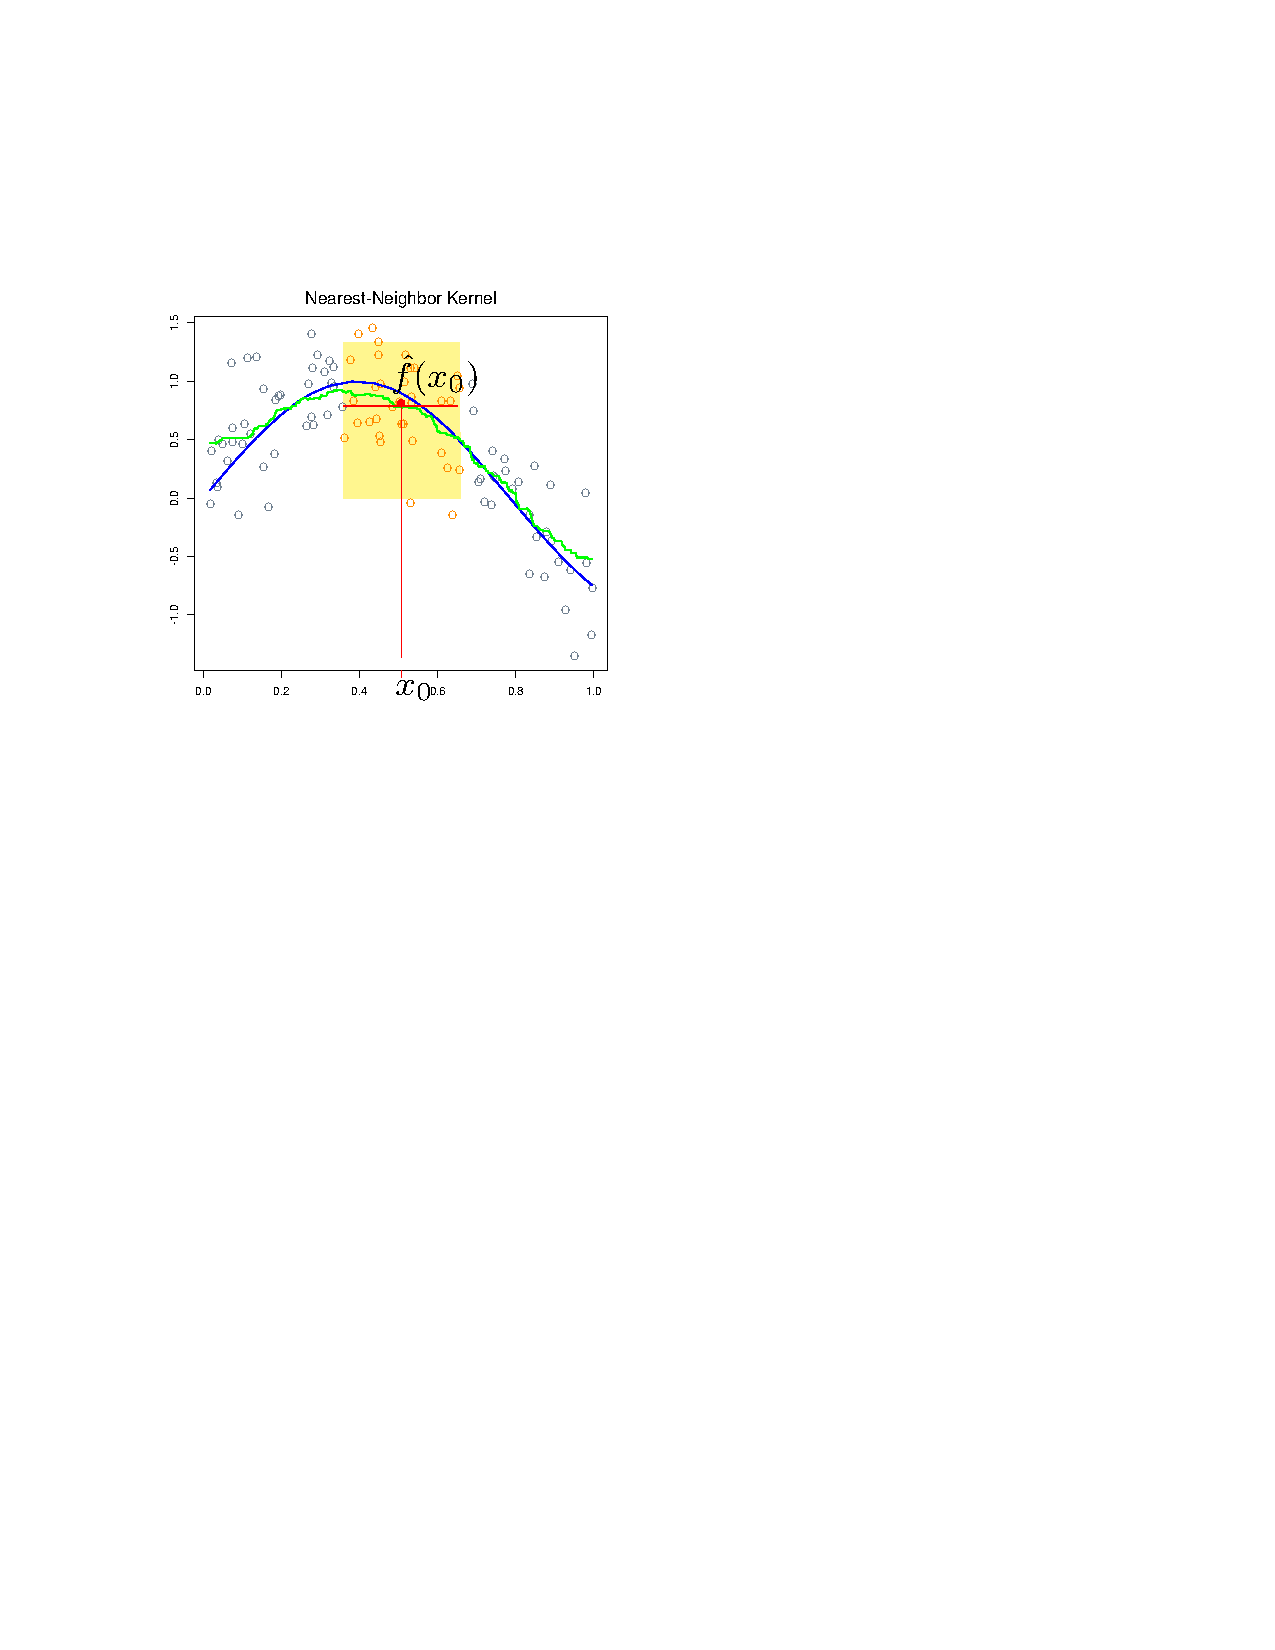
\includegraphics[width=\textwidth]{figures/knn.pdf}
        \end{figure}
\end{columns}
\end{frame}


\begin{frame}
\frametitle{Improving on $k$NN}
\begin{columns}
\column{0.65\textwidth}
    \begin{itemize}
        \item $k$NN gives equal weight to all points that falls within the $k$ nearest neighbor region.
        \item Solution: use a weighted kernel that goes to zero smoothly with distance from point.
        \item Nadaraya-Watson kernel-weighted average:
        \begin{equation*}
            \hat{f}(x) = \frac{\sum_{i=1}^N K_{\lambda}(x_0,x_i)y_i}{\sum_{i=1}^N K_{\lambda}(x_0,x_i)}
        \end{equation*}
        \item Epanechnikov quadratic kernel:
        \begin{equation*}
            K_{\lambda}(x_0,x) = D(\frac{|x-x_0|}{\lambda}), D(t) = \frac{3}{4}(1-t^2)\mathrm{~if~}|t| \leq 1
        \end{equation*}
    \end{itemize}
\column{0.35\textwidth}
\begin{figure}
            \centering
            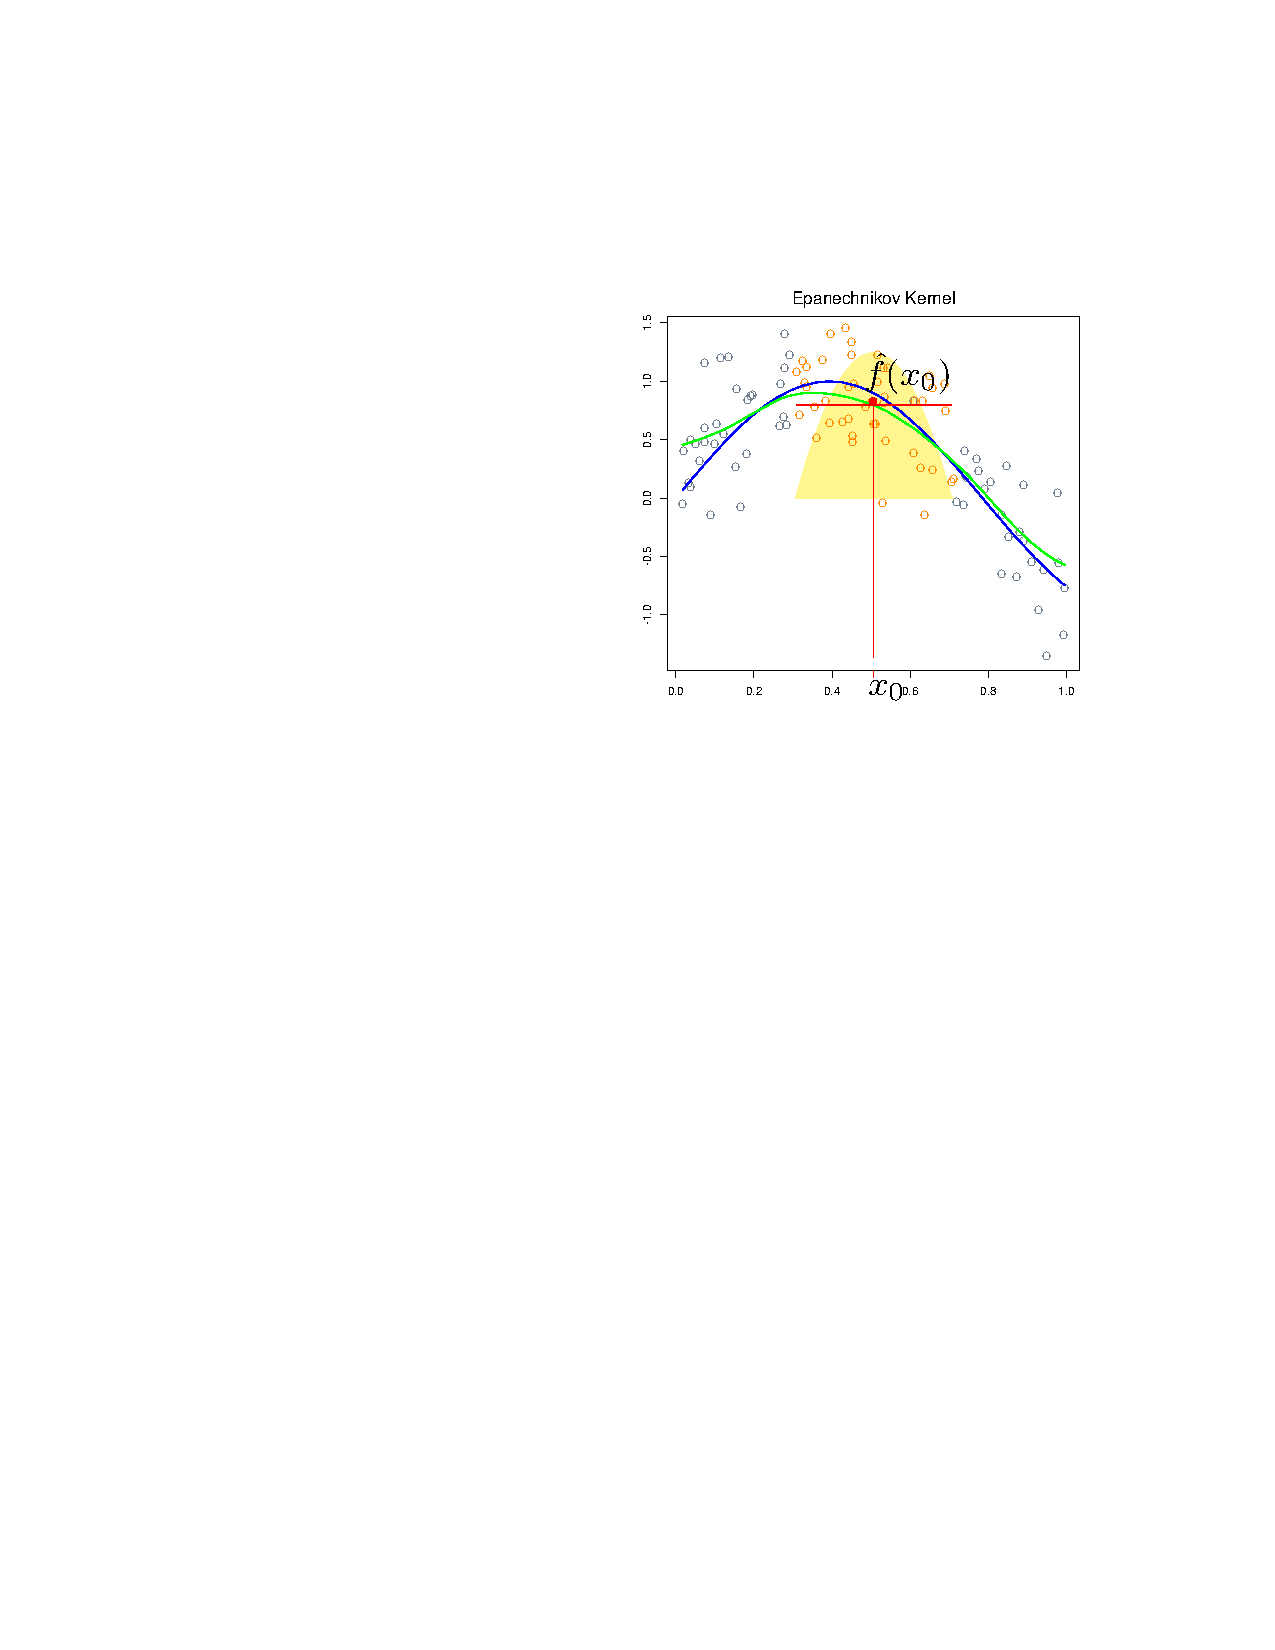
\includegraphics[width=\textwidth]{figures/epankernel.pdf}
        \end{figure}
\end{columns}
\end{frame}


\begin{frame}{Considerations}
    \begin{itemize}
        \item Smoothing parameter $\lambda$ determines the width of the local neighborhood. Large $\lambda$ means lower variance but higher bias.
        \item Metric window widths: As local density increases, vias decreases.
        \item Epanechnikov kernel is compact. Tri-cube kernel $D(t) = (1-|t|^3)^3\mathrm{~if~}|t| \leq 1$ is another compact kernel that is flatter and differentiable at bounday.
        \item Gaussian kernel is a popular \textit{non-compact} kernel. Standard deviation controls width of kernel.
        \begin{figure}
            \centering
            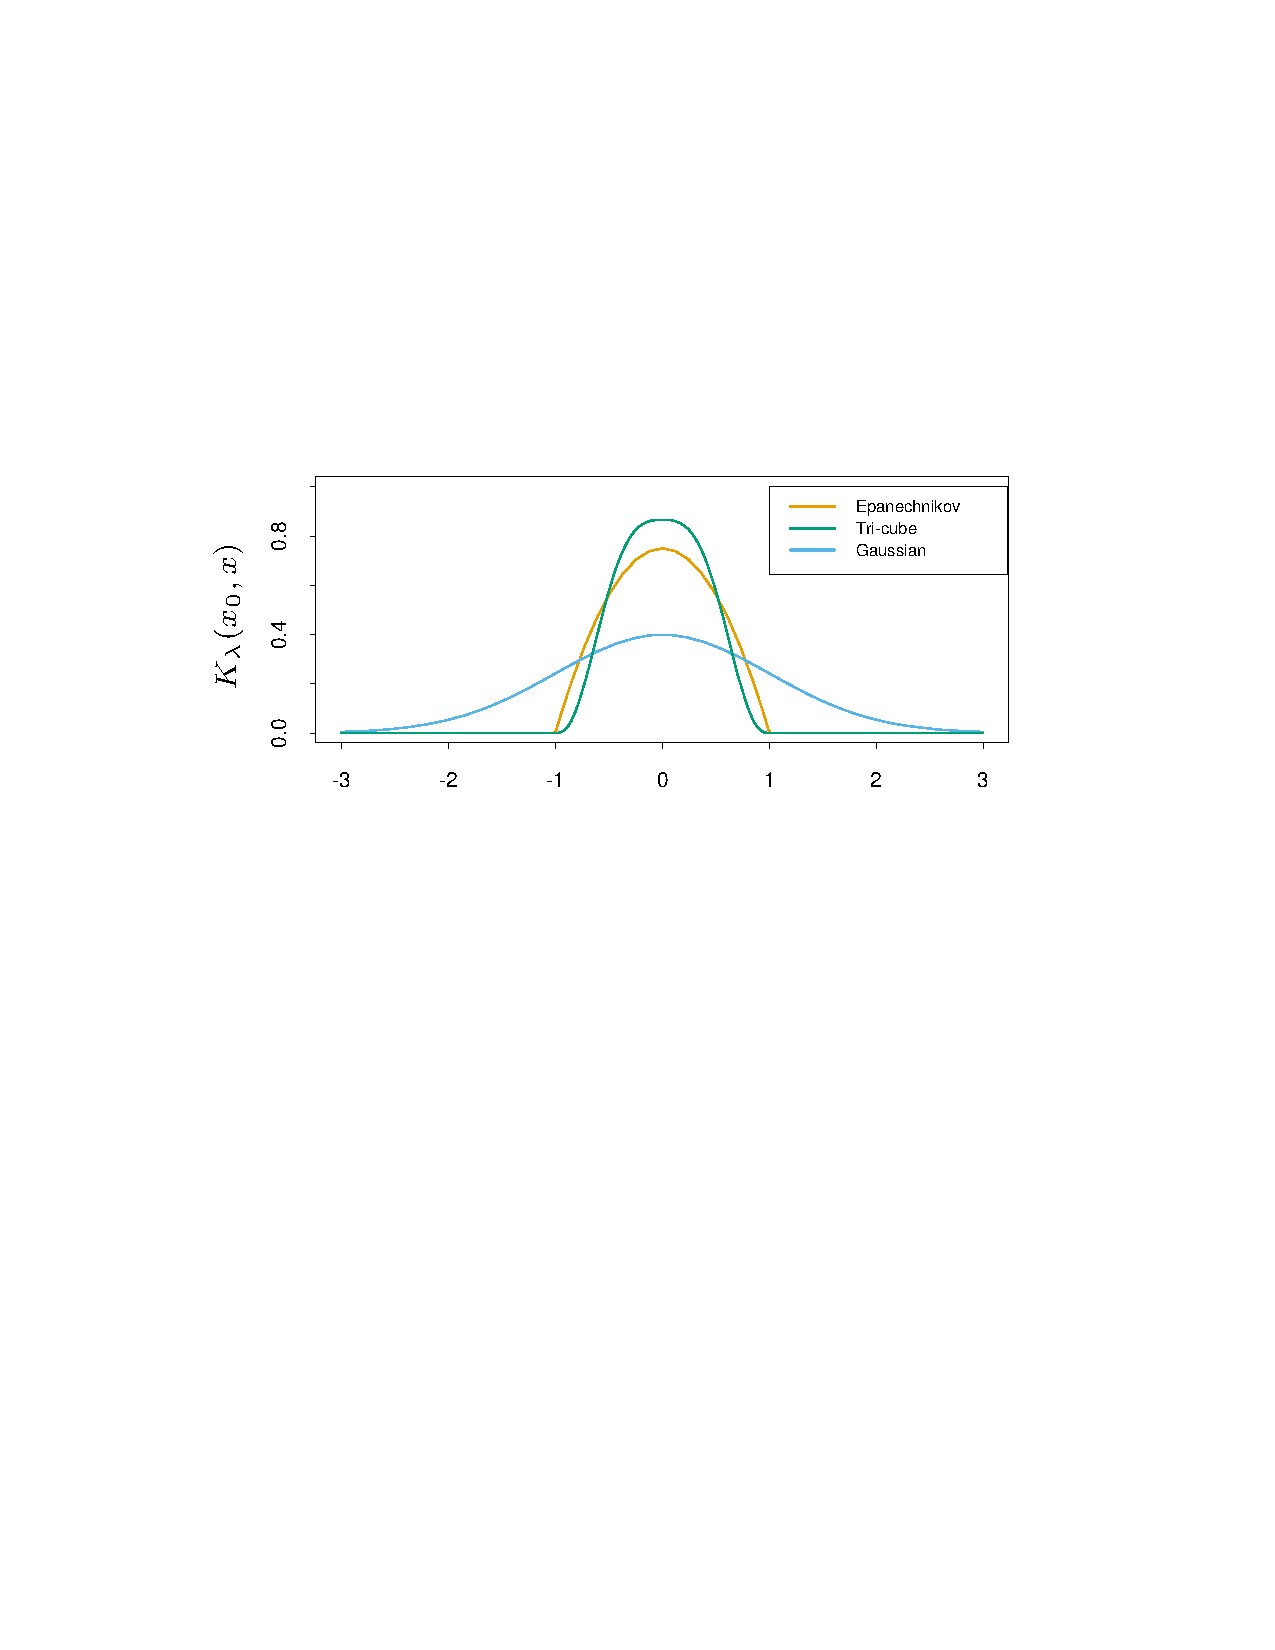
\includegraphics[width=0.5\textwidth]{figures/kerneltypes.pdf}
        \end{figure}
    \end{itemize}
\end{frame}


\begin{frame}[fragile]{Code}
\inputminted{python}{example_knn.py}
\end{frame}


\begin{frame}{Local linear/polynomial regression}
    \begin{itemize}
        \item Local linear/polynomial regression can be used, which corrects bias at boundary regions at the expense of higher variance. 
        \item For higher dimensions especially, local linear regression is preferred to local constant fit.
        \begin{figure}
            \centering
            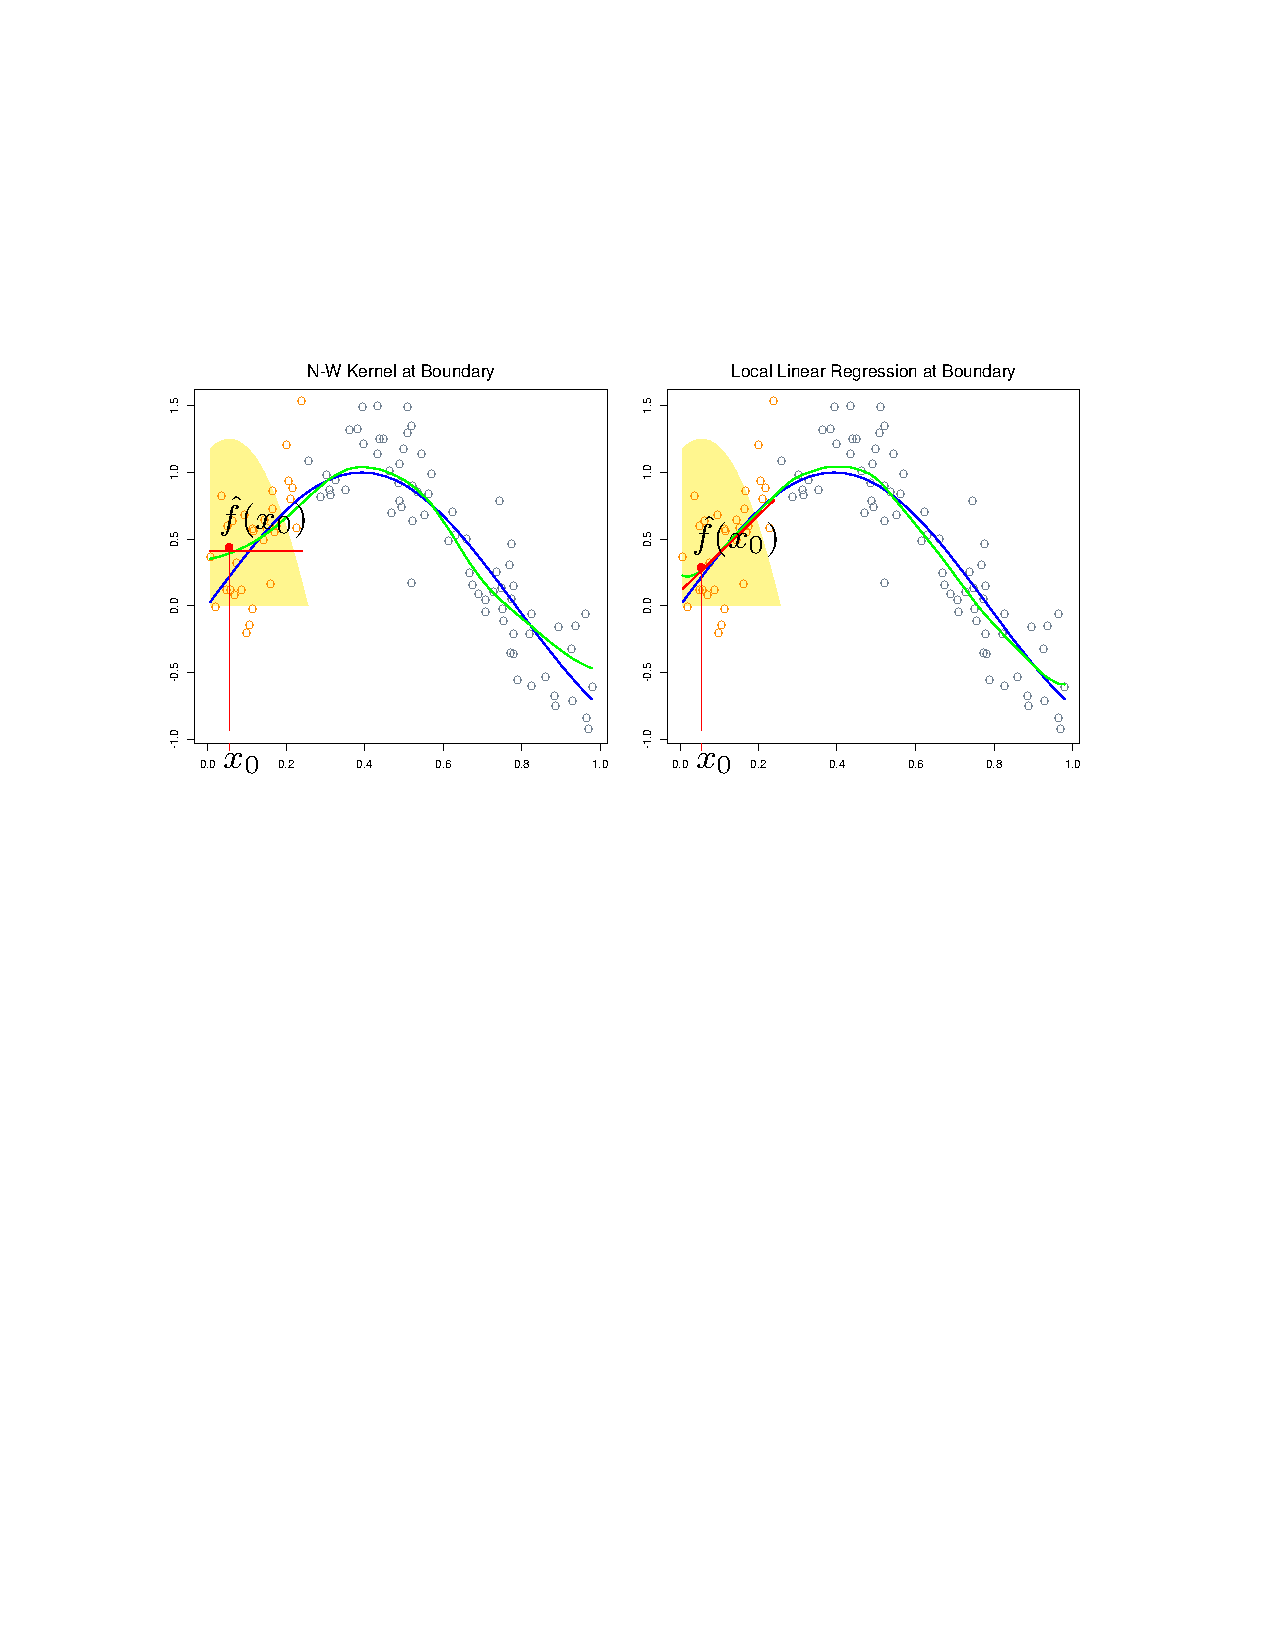
\includegraphics[width=0.6\textwidth]{figures/localkernelregression.pdf}
        \end{figure}
        \item Often used to interpolate within a region of feature space.
    \end{itemize}
\end{frame}


\section{Kernel Density Estimation}


\begin{frame}{Kernel Density Estimation}
    \begin{itemize}
        \item Estimate the probability density function $\hat{f}_X(x)$ as:
        \begin{equation*}
            \hat{f}_X(x_0) = \frac{\# x_i \in N(x_0)}{N\lambda}
        \end{equation*}
        where $\lambda$ is the width of the bin and $N(x_0)$ is the neighbor of $x_0$ and $N$ is the total data count.
        \item Often, the smooth Parzen estimate is used.
        \begin{equation*}
            \hat{f}_X(x_0) = \frac{1}{N\lambda}\sum_{i=1}^{N} K_{\lambda}(x_0, x_i)
        \end{equation*}
        \item Popular choice of $K_{\lambda}$ is the Gaussian kernel $\phi(\frac{x-x_0}{\lambda})$.
        \item Essentially $f_X(x)$ is the convolution of the sample distribution with the Gaussian distribution with standard deviation $\lambda$.
    \end{itemize}
\end{frame}


\begin{frame}{Gaussian KDE}
\begin{figure}
    \centering
    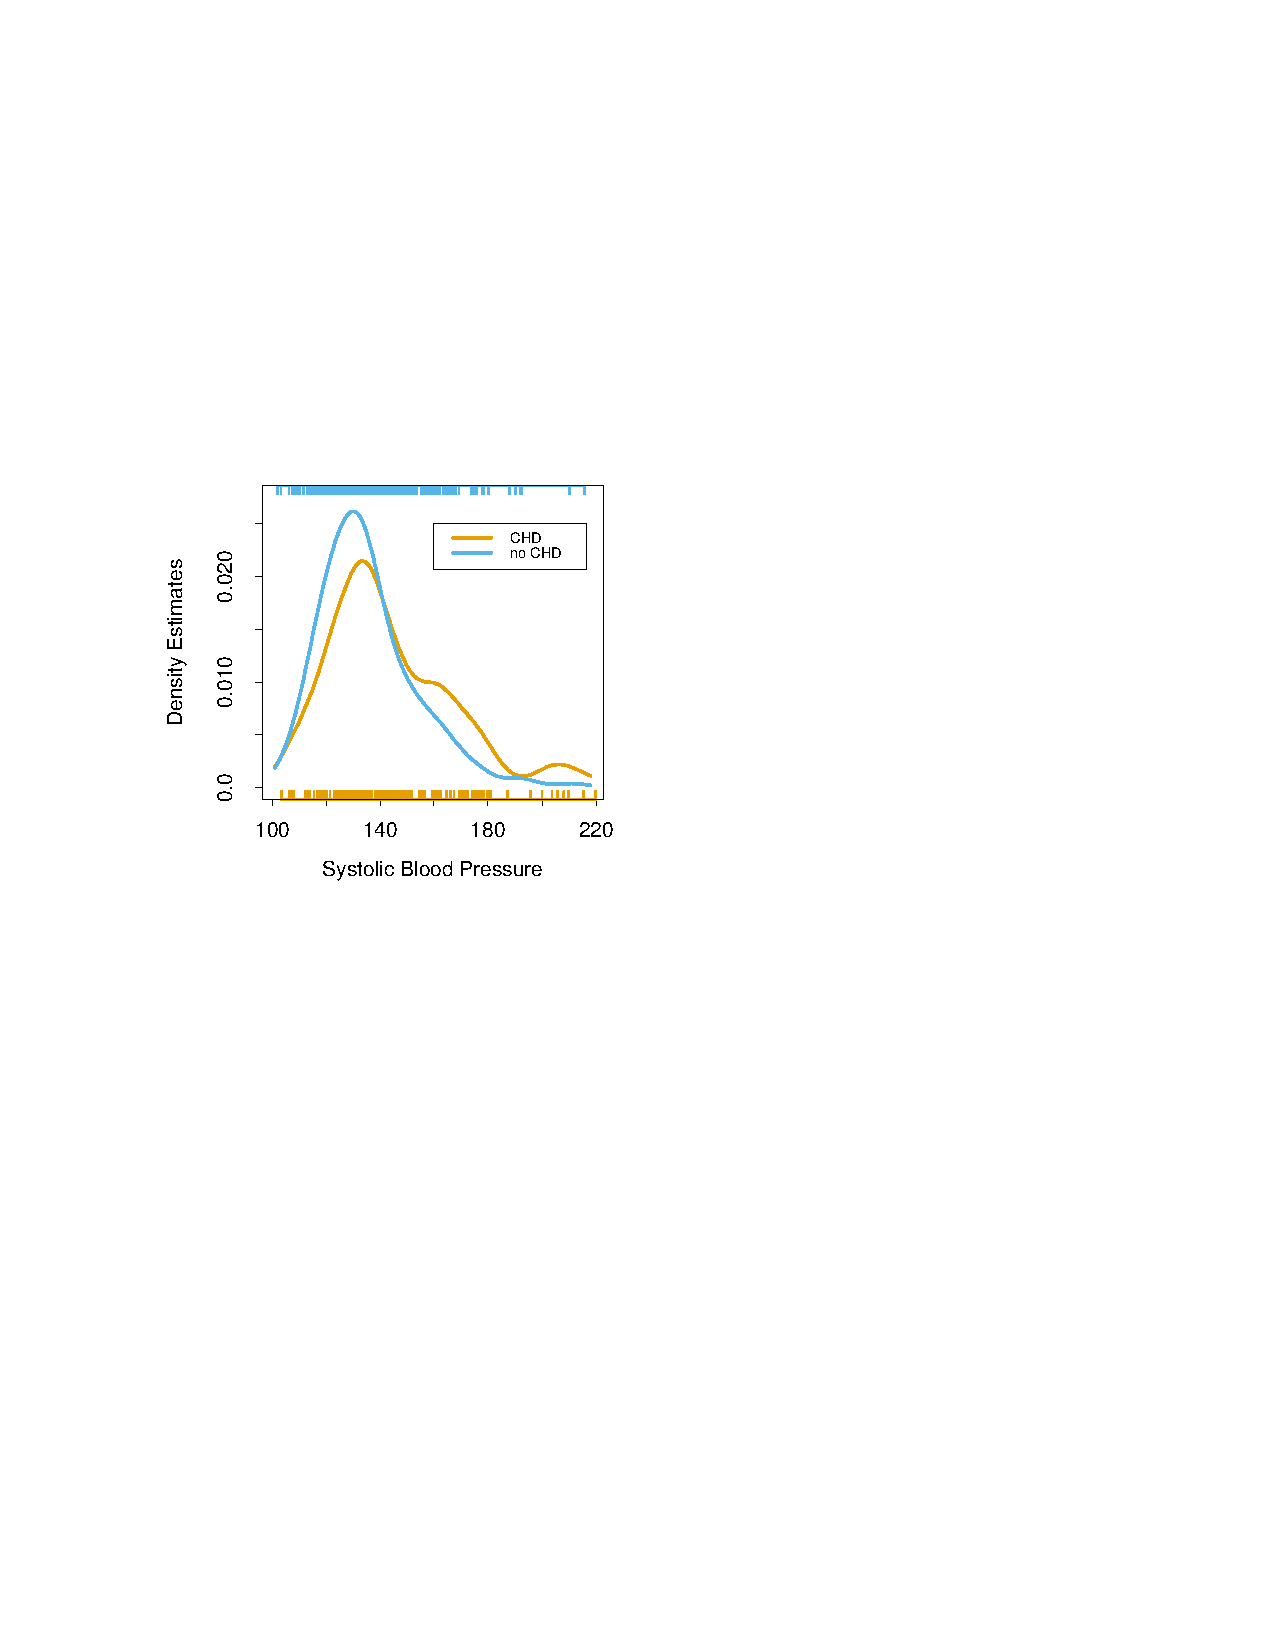
\includegraphics[width=0.45\textwidth]{figures/gaussian_kde.pdf}
\end{figure}
\end{frame}


 \begin{frame}{Example of Gaussian Density Estimation in Interatomic Potential}
    \begin{itemize}
        \item Gaussian Approximation Potential\cite{bartokGaussianApproximationPotentials2010} uses a smooth-overlap of atomic positions (SOAP) kernel in a Gaussian process model:
    \begin{eqnarray*}
        \rho_{i}(\boldsymbol{R}) = \sum_{j} f_{c}(R_{ij}) \cdot \exp(-\frac{|\boldsymbol{R} - \boldsymbol{R}_{ij}|^{2}}{2\sigma_{\rm atom}^{2}}) = \sum_{nlm} c_{nlm} \ g_{n}(R) Y_{lm}(\hat{\boldsymbol{R}}),
    \end{eqnarray*}
    \end{itemize}
    \begin{figure}
        \centering
        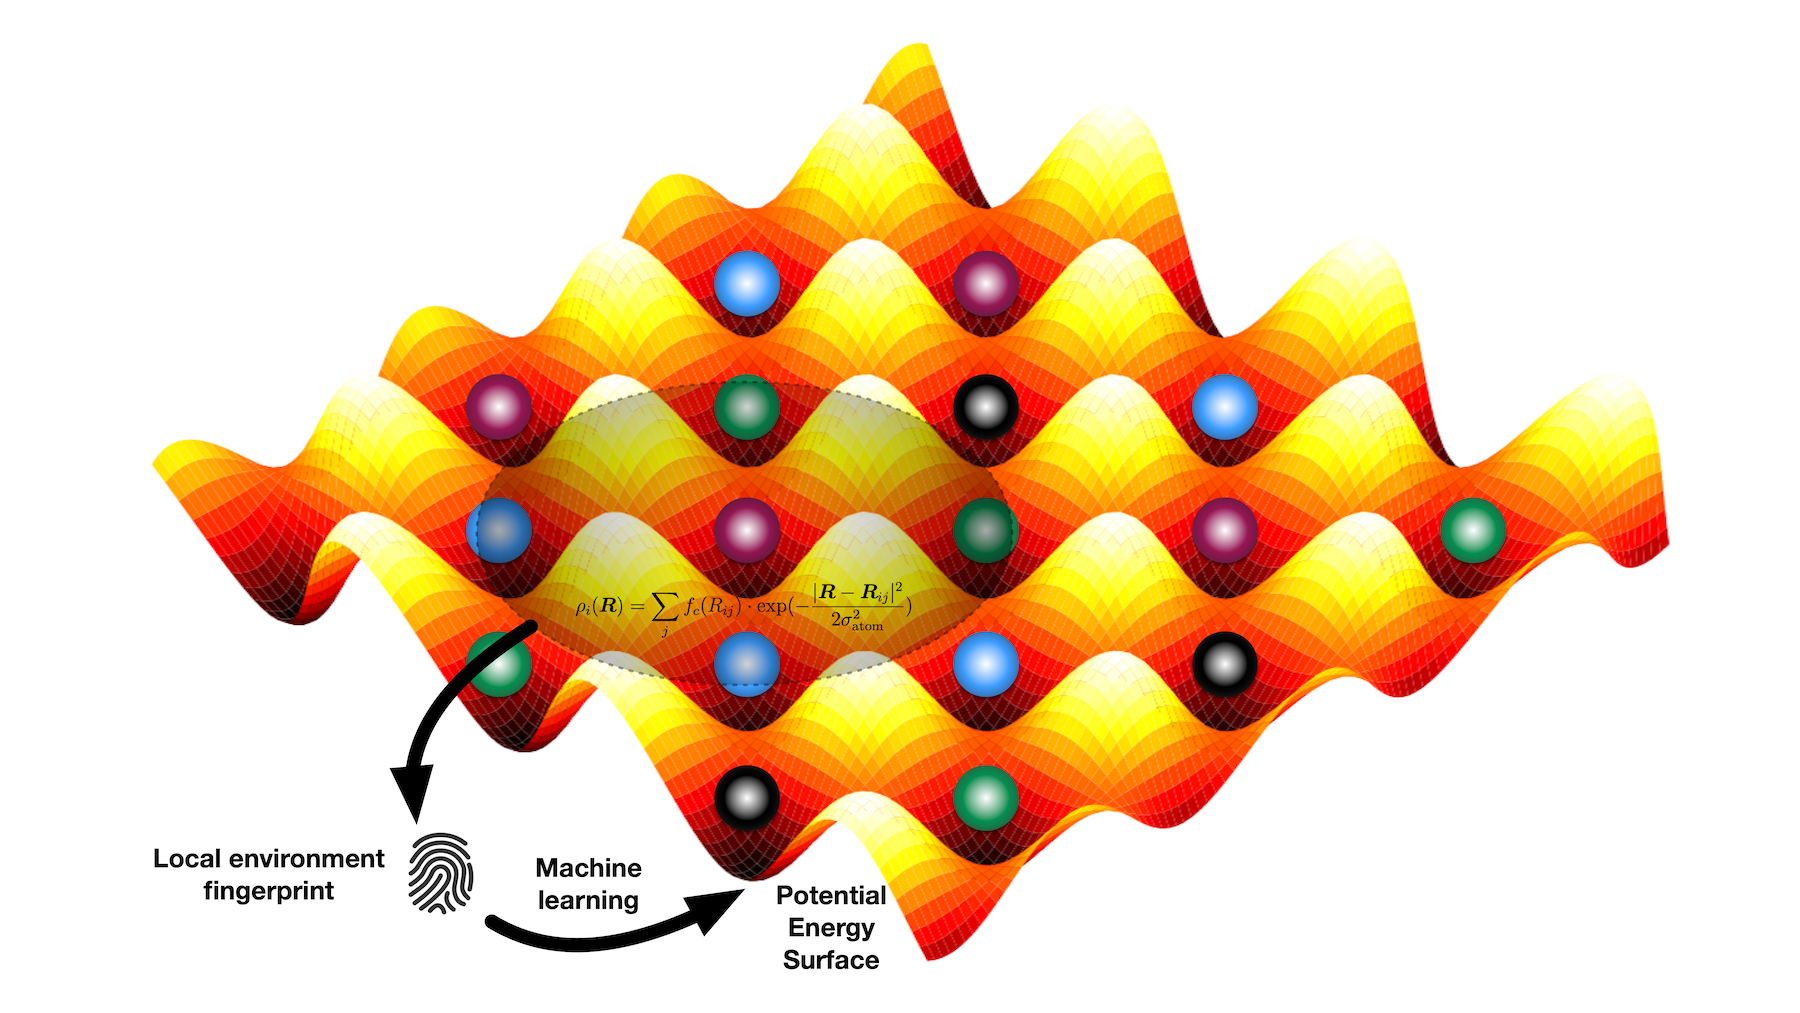
\includegraphics[width=0.45\textwidth]{figures/PES.png}
    \end{figure}
\end{frame}


\section{Kernel Density Classification}

\begin{frame}{Kernel Density Classification}
    \begin{itemize}
        \item Given the kernel density estimate for each class $\hat{f}_j(X)$ and class prior $\pi_j$, we can use Bayes theorem to perform classification:
        \begin{equation*}
            P(G=j|X=x_0) = \frac{\pi_j \hat{f}_j(x_0)}{\sum_{k=1}^J\pi_k \hat{f}_k(x_0)}
        \end{equation*}
        \item However, density estimation for each class is not necessary if we only need to perform classification.
        \item The key is to estimate the posterior decision boundary between classes accurately.
    \end{itemize}
    \begin{figure}
        \centering
        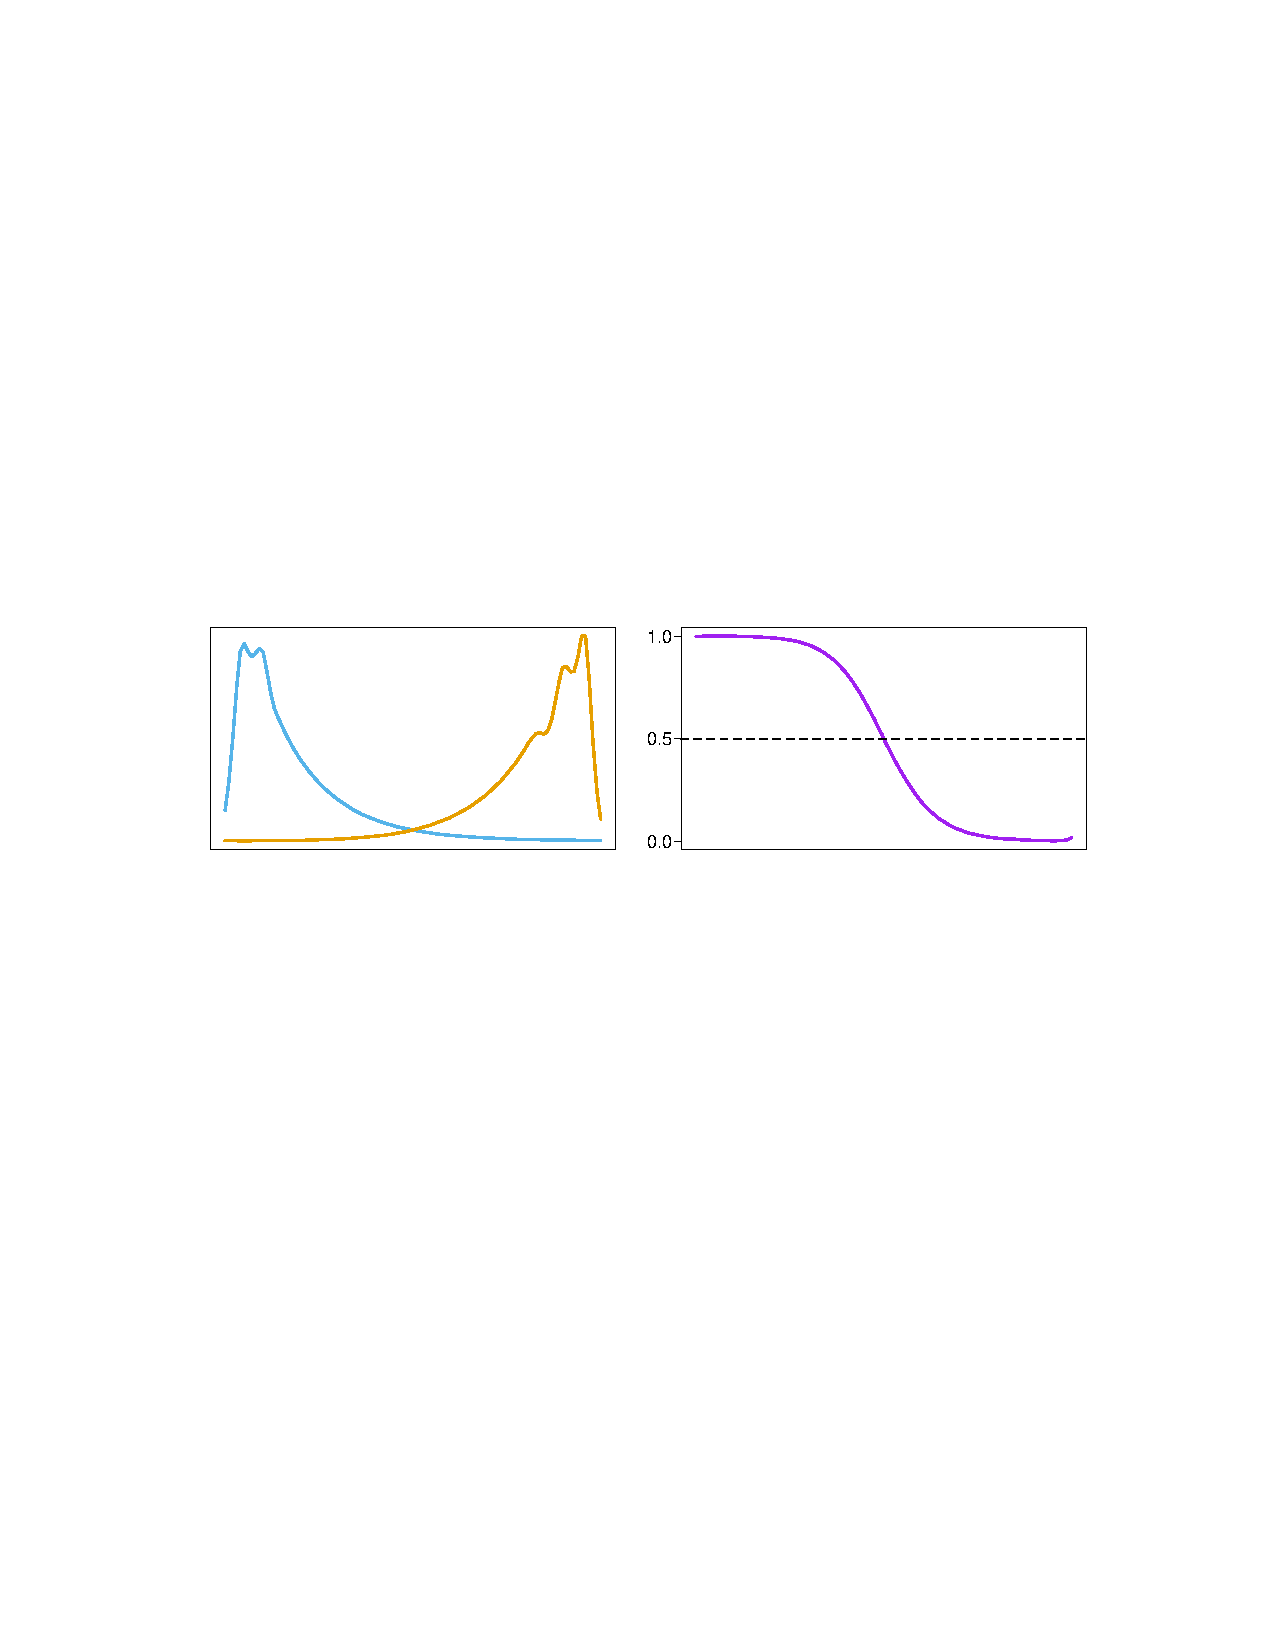
\includegraphics[width=0.6\textwidth]{figures/classdensities.pdf}
    \end{figure}
\end{frame}


\begin{frame}{Naive Bayes}
    \begin{itemize}
        \item Highly popular approach and often outperforms more sophisticated alternatives.
        \item Assumes features $X_k$ are independent, i.e., $f_j(X) = \prod_{k=1}^p f_jk(X_k)$, i.e., class conditional probabilities can be estimated using 1D kernel densities!
        \begin{eqnarray*}
        \log{\frac{P(G=l|X)}{P(G=k|X)}} & = & \log{\frac{\pi_l}{\pi_j}} + \sum_{k=1}^p \log{\frac{f_{lk}(X_k)}{f_{jk}(X_k)}}\\
        & = & \alpha_l + \sum_{k=1}^p g_{lk}(X_k)
        \end{eqnarray*}
        We are converting a high-dimensional problem into simpler generalized additive model (see later lecture on GAMs). 
    \end{itemize}
\end{frame}


\begin{frame}{Radial Basis Functions}
    \begin{itemize}
        \item Treat kernel functions as basis functions.
        \begin{equation*}
            f(x) = \sum_{j=1}^M D(\frac{||x-\varepsilon_j||}{\lambda_j})\beta_j
        \end{equation*}
        \item Each basis function is index by location ($\varepsilon_j$) and scale parameter $\lambda_j$.
        \item Gaussian function is a common choice for $D$.
        \item Parameters are optimized, typically using a least squares approach.
    \end{itemize}
\end{frame}


\begin{frame}{Mixture Models}
    \begin{itemize}
        \item Type of kernel model.
        \begin{equation*}
            f(x) = \sum_{m=1}^M \alpha_m \phi(x; \mu_m, \vec{\Sigma_m})
        \end{equation*}
        \item Again, Gaussian mixture model is by far the most common choice.
        \item If covariance matrices are constrained to be scalars. then it is similar to a radial basis expansion.
        \item Typically fitted using maximum likelihood approach / expectation maximization (next lecture).
        \item Probability that observation $i$ belongs in component $m$ is given by:
        \begin{equation*}
            \hat{r}_{im} = \frac{\alpha_m \phi(x; \mu_m, \vec{\Sigma_m})}{\sum_{k=1}^M \alpha_k \phi(x; \mu_k, \vec{\Sigma_k})}
        \end{equation*}
        \item Very often used in spectroscopy analysis.
    \end{itemize}
\end{frame}


\begin{frame}{CARS spectroscopy analysis using Gaussian Mixtures}
\begin{figure}
    \centering
    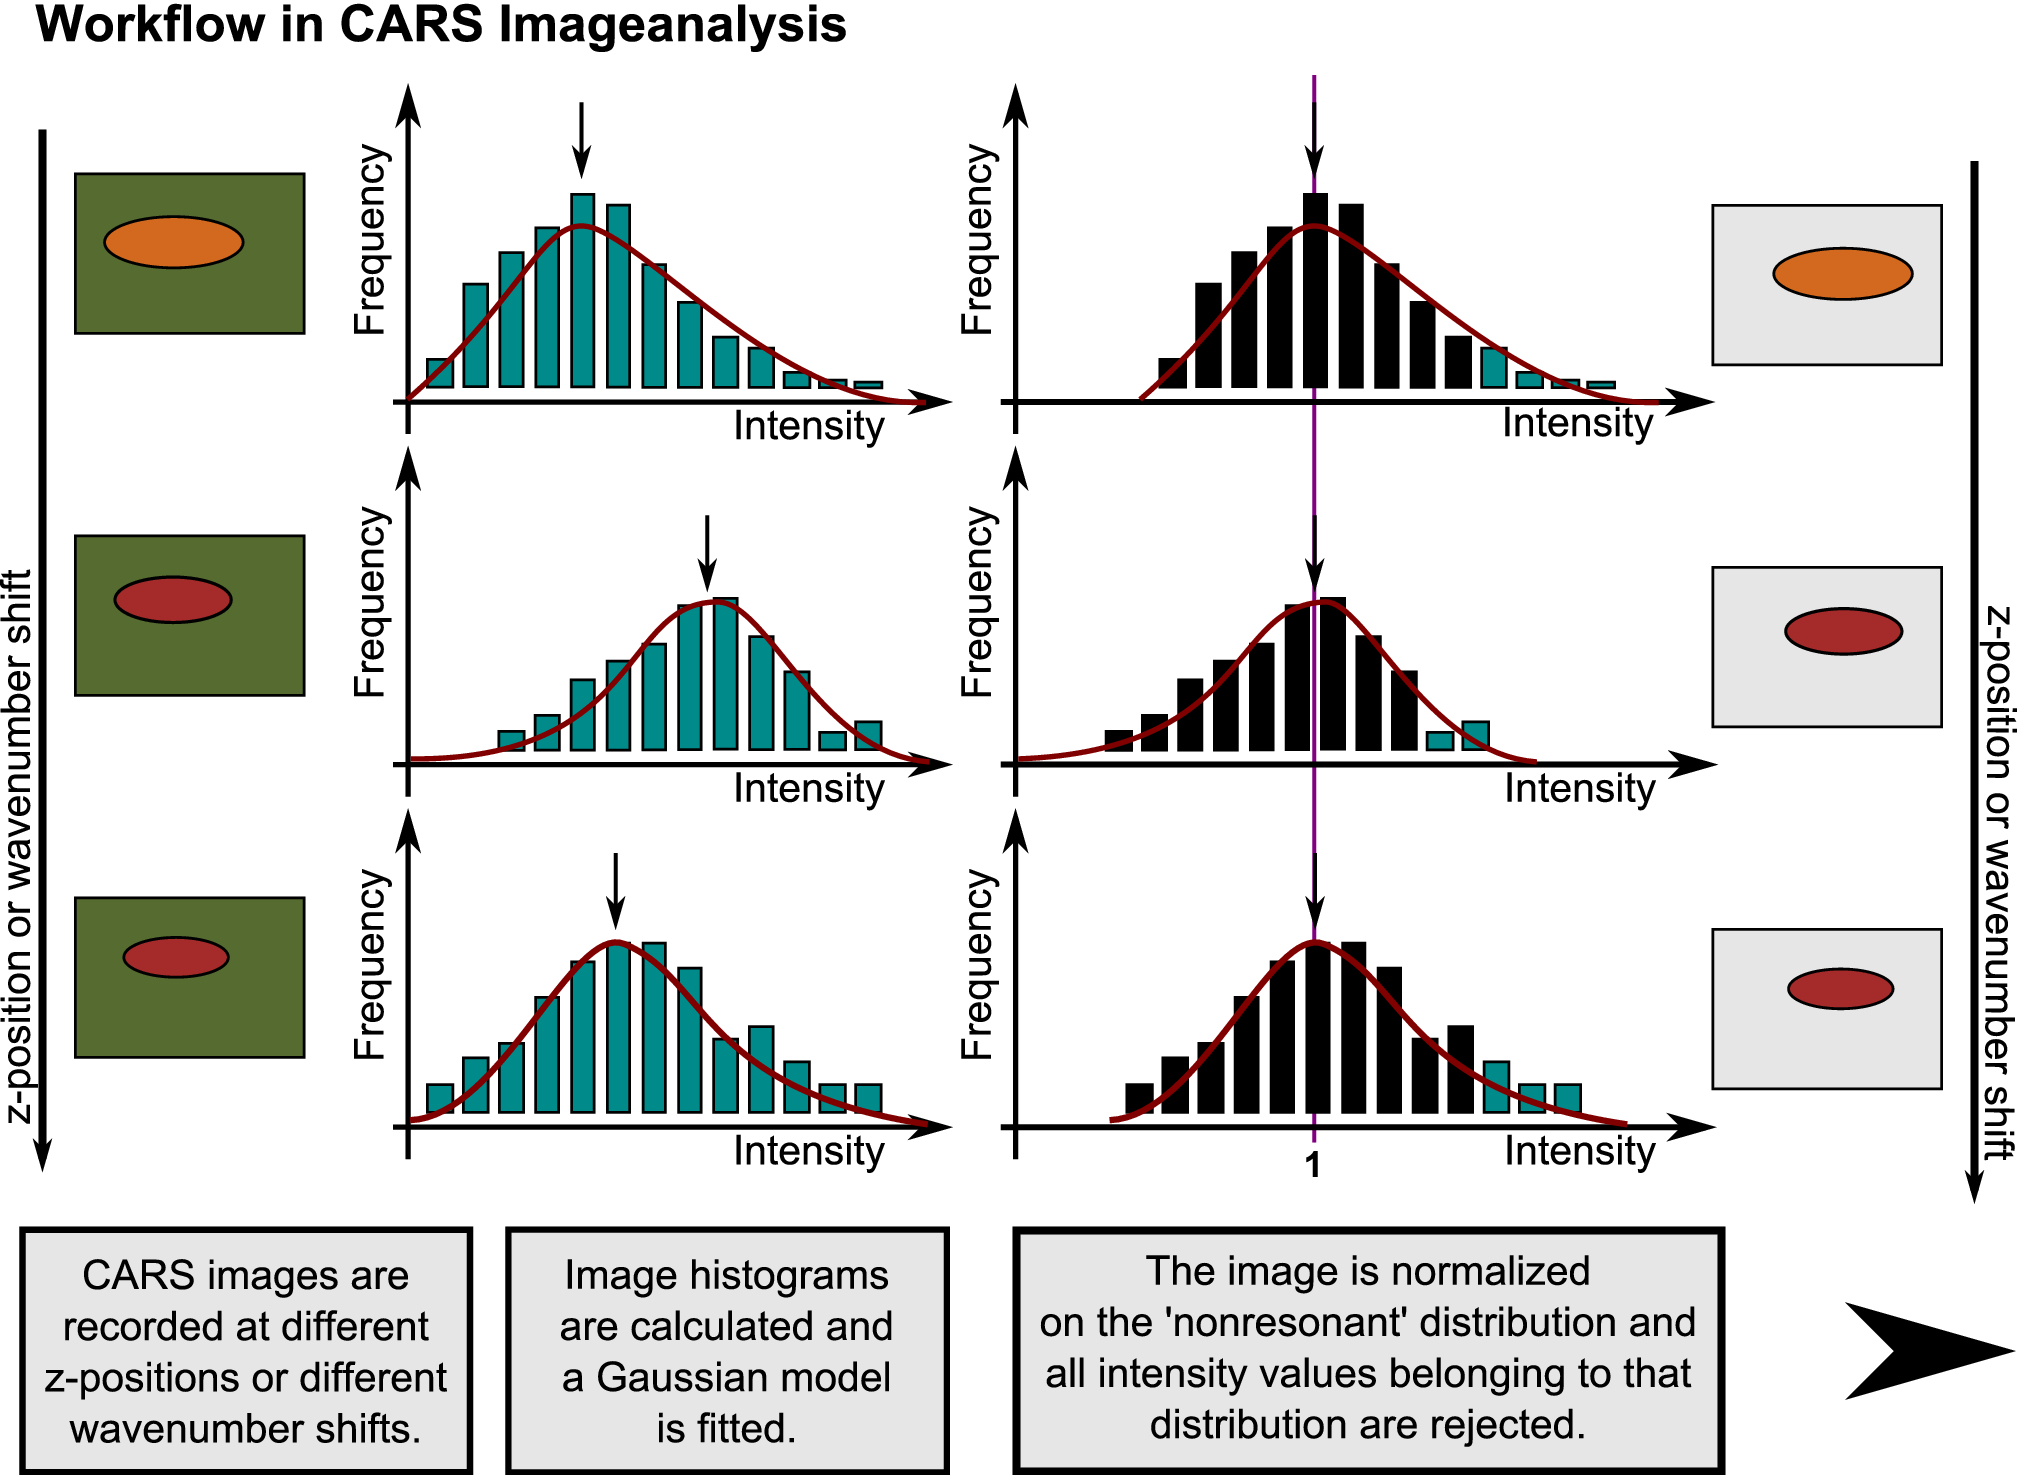
\includegraphics[width=0.3\textwidth]{figures/cars1.jpeg}
    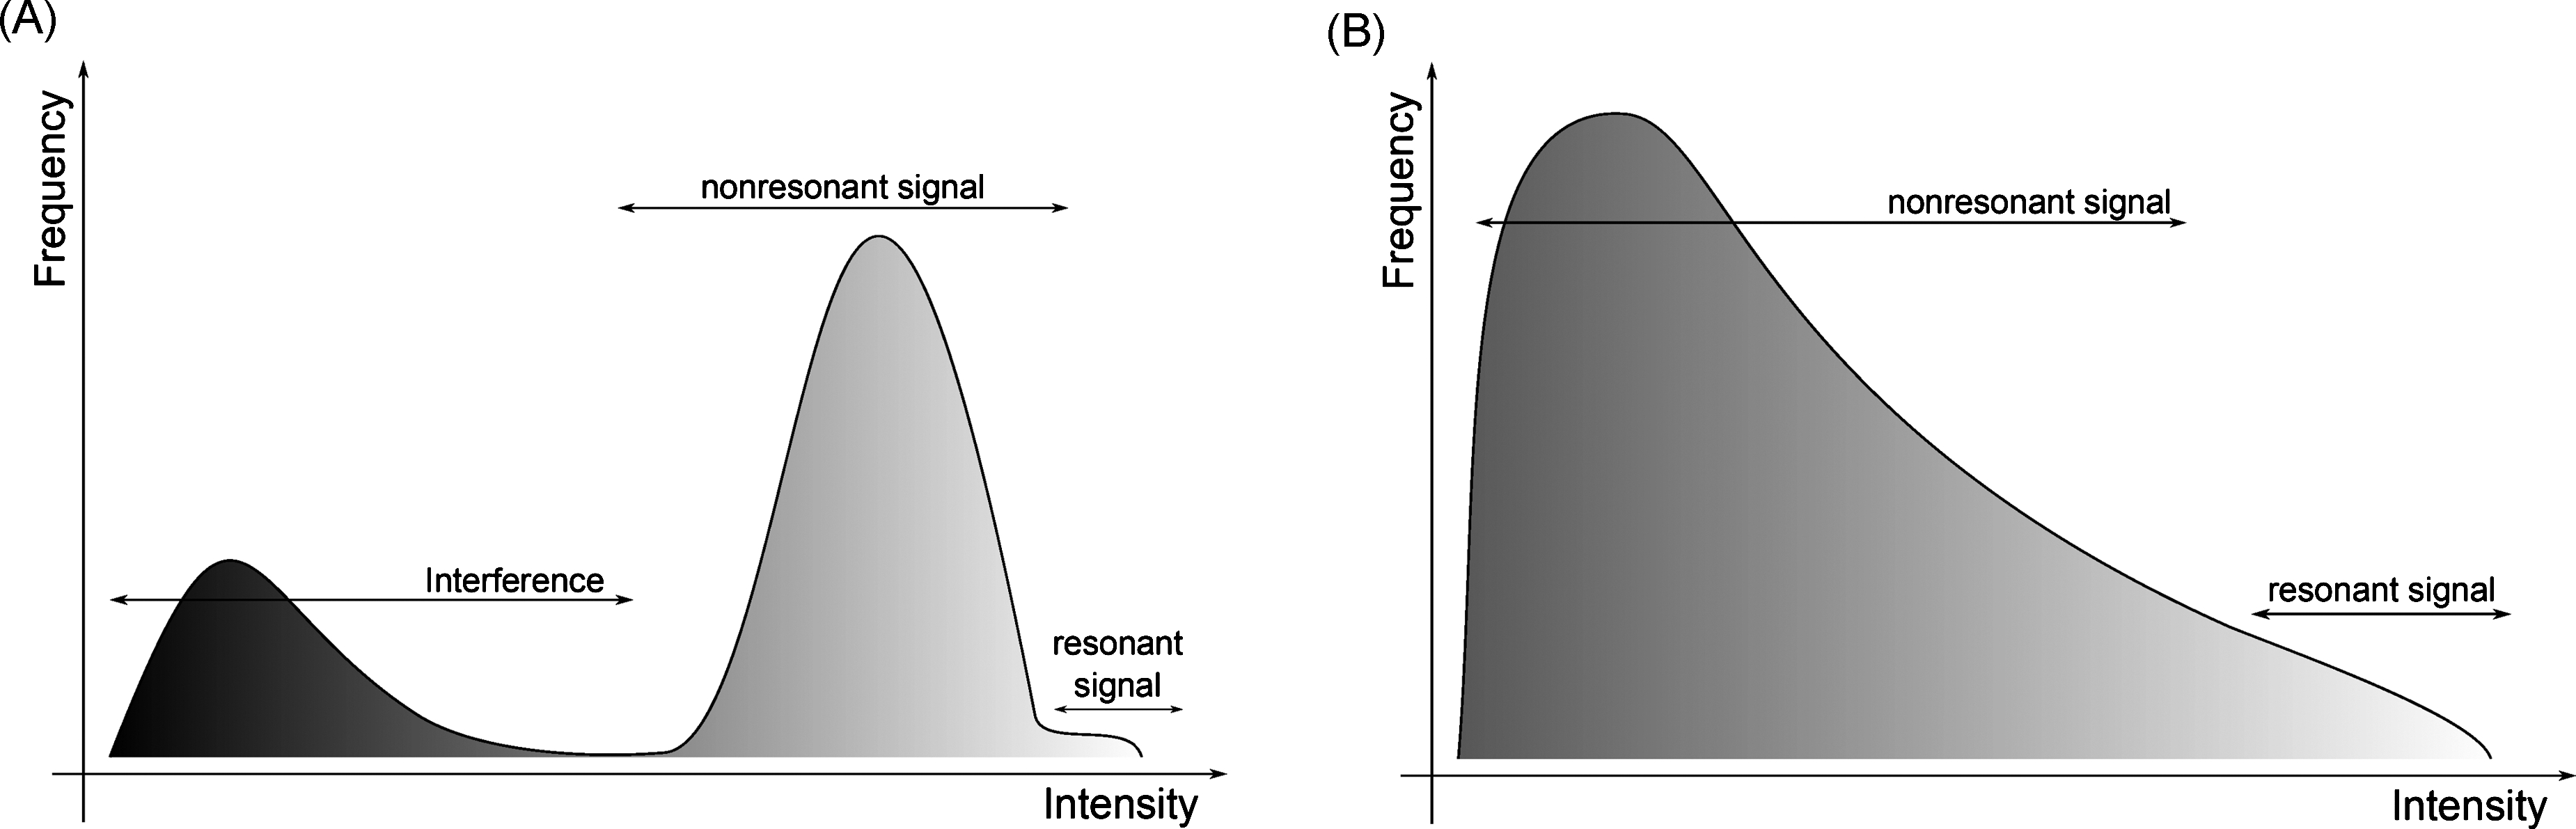
\includegraphics[width=0.65\textwidth]{figures/cars2.jpeg}
    \caption{From ref. \cite{voglerSeparationCARSImage2010}}
\end{figure}
\end{frame}


\begin{frame}{Bibliography}
    \bibliographystyle{unsrt}
    \bibliography{refs}
\end{frame}




\begin{frame}
    \Huge{\centerline{The End}}
\end{frame}

\end{document}

